\chapter{Berechenbarkeitstheorie}
\begin{description}
\item[Algorithmus] $A: \Sigma_{\tx{Input}}^* \ra \Sigma_{\tx{Output}}^*$\\
		Algorithmus ist eine Verfahren, dass
		\begin{itemize}
		\item Eingabew�rter schrittweise verarbeitet (deterministisch).
		\item durch einen endlichen Text bis ins letzte Detail eindeutig festgelegt ist.
		\item bei Terminierung eine Ausgabe liefert, oder nicht determiniert.
		\end{itemize}
\end{description}
Wozu formales Modell, wenn wir Algorithmen auch so (\ac{z.B.} Programmiersprache) beschreiben k�nnen?
\begin{itemize}
\item geht es um Berechenbarkeit reicht intuitives Vorgehen f�r positive Antwort aus, da Programmier Sprachen eindeutige Semantik hat
\item negative Antwort ohne formales Modell nur schwer zu zeigen
\end{itemize}
Anforderungen an formales Modell
\begin{itemize}
\item einfach, um formale Beweise zu erleichtern
\item berechnungsuniversell; \ac{d.h.} alle intuitiv berechenbaren Funktionen werden erfasst.
\end{itemize}

\begin{fdefinition}
\Insert{GI-23.06.2009-IMG-1}
Eine \ac{TM} ist ein 7-Tupel
\[M = \rkl{Q, \Sigma, \Gamma, \delta, q_0, q_{\tx{accept}}, q_{\tx{reject}}}\]
mit
\begin{itemize}
\item einer endlichen Zustandsmenge $Q$
\item einem Eingabealphabet $\Sigma$, wobei das \indexb{Randsymbol} \ggq{$\cent$}\index{$\cent$ Randsymbol} und das Leerzeichen \ggq{\textvisiblespace} nicht in $\Sigma$ enthalten sind
\item einem Ausgabealphabet $\Gamma$, wobei $\Sigma \subseteq \Gamma$ und $\gklamm{\cent, w} \subseteq \Gamma$.
\item einer �bergangsfunktion
		\[\delta:~ Q - \gklamm{q_{\tx{accept}}, q_{\tx{reject}}} \times \Gamma \ra Q \times \Gamma \times \gklamm{L, R, N}\]
		mit der Eigenschaft
		\[\forall q \in Q:~\delta\rkl{q, \cent} \in Q \times \gklamm{\cent} \times \gklamm{R, N}\]
		was bedeutet das man kein $\cent$ auf das Band schreiben kann.

\item einem Startzustand $q_0 \in Q$
\item einem akzeptierenden Zustand $q_{\tx{accept}} \in Q$
\item einem verwerfenden Zustand $q_{\tx{reject}} \in Q$
\end{itemize}
$\delta(q, a) = \rkl{q_1, b, L}$ bedeutet, dass die \ac{TM} im Zustand $q$ durch Lesen des Symbols $a$ in den Zustand $q_1$ �bergehen kann, das Symbole $a$ durch $b$ ersetzt und den \ac{S-/L-Kopf} eine Position nach links bewegt.
\Mark{Definition 5.1}
\end{fdefinition}
\begin{fdefinition}
Sei $M = \rkl{Q, \Sigma, \Gamma, \delta, q_0, q_{\tx{accept}}, q_{\tx{reject}}}$ eine \ac{TM}. Eine Konfiguration $C$ von $M$ ist ein Element aus
\[\Konf{(M)} = \gklamm{\cent} \mal \Gamma^* \mal Q \mal \Gamma^+ \cup Q \mal \gklamm{\cent} \mal \Gamma^*\]
F�r ein Wort $w \in \Sigs$ ist $q_0 \cent w$ eine Startkonfiguration; eine Konfiguration der Gestalt $v_1 q_{\tx{accept}} v_2$ hei�t akzeptierende Konfiguration und eine Konfiguration der Gestalt $v_1 q_{\tx{reject}} v_2$ hei�t verwerfende Konfiguration $\rkl{v_1, v_2 \in \Gamma^*}$. Eine Konfiguration $v_1 q a v_2$ mit $v_1, v_2 \in \Gamma^*$, $a \in \Gamma$, $q \in Q$ beschreibt folgende Situation.
\begin{itemize}
\item \ac{TM} befindet sich im Zustand $q$
\item auf dem Band steht $v_1 a v_2$, wobei $v_1 = \cent v_1'$ $v_1' \in \Gamma^*$ gefolgt von unendlich vielen Blank-Symbolen \textvisiblespace
\item der \ac{S-/L-Kopf} befindet sich auf dem $\rkl{\betrag{v_1} + 1}$-ten Feld des Bandes und liefert $a$ als n�chstes Symbol.
\end{itemize}
\Mark{Definition 5.2}
\end{fdefinition}
\begin{fdefinition}
Sei $M = \rkl{Q, \Sigma, \Gamma, \delta, q_0, \qacc, \qrej}$ eine \ac{TM}. Ein Konfigurations�bergang (ein Schritt) von $M$ ist eine Relation $\vd:~\Konf{(M)} \times \Konf{(M)}$, die \ac{def.} ist durch
\begin{enumerate}
\item \ac{S-/L-Kopf} bleibt $\rkl{\delta \rkl{q, a_i} = \rkl{p, b, N}}$
		\[a_1 a_2 \dots a_{i - 1} \textcolor{red}{q} \textcolor{blue}{a_i} a_{i + 1} \dots a_n \vd_{M} a_n \dots a_{i - 1} \txcol{red}{p} \txcol{blue}{b} a_{i + 1} \dots a_n\]

\item \ac{S-/L-Kopf} geht nach links $\rkl{\delta \rkl{q, a_i} = \rkl{p, b, L}}$
		\[a_1 a_2 \dots a_{i - 1} \txcol{red}{q} \txcol{blue}{a_i} a_{i + 1} \dots a_n \vd_{M} a_1 \dots a_{i - 2} \txcol{red}{p} a_{i - 1} \txcol{blue}{b} a_{i + 1} \dots a_n\]

\item \ac{S-/L-Kopf} geht nach rechts $\rkl{\delta \rkl{q, a_i} = \rkl{p, b, R}}$
		\begin{enumerate}
		\item Kopf auf letztem Zeichen
				\[a_1 a_2 \dots a_{n - 1} \txcol{red}{q} \txcol{blue}{a_n} \vd_M a_1 a_2 \dots a_{n - 1} \txcol{blue}{b} \txcol{red}{p} \tx{\textvisiblespace}\]

		\item Kopf nicht auf letztem Zeichen
				\[a_1 a_2 \dots a_{i - 1} \txcol{red}{q} \txcol{blue}{a_i} \dots a_n \vd_M a_1 a_2 \dots a_{i - 1} \txcol{blue}{b} \txcol{red}{p} a_{i + 1} \dots a_n\]
		\end{enumerate}
		nennen wir Schrittrelation.
\end{enumerate}
\Mark{Definition 5.3}
\end{fdefinition}
\begin{fdefinition}
Sei $M = \rkl{Q, \Sigma, \Gamma, q_0, \qacc, \qrej}$ eine \ac{TM} und $w \in \Sigs$. Eine Berechnung ist eine, m�glicherweise unendliche, Kette von Konfigurationen:
\[C = C_0 C_1 \dots\]
mit $C_i \in \Konf{(M)}$ und $C_i \vd_M C_{i + 1}$ ($i \in \N$). Ist die Berechnung endlich so endet sie in einer Konfiguration $C_n = v_1 q v_2$ mit $q \in \gklamm{\qacc, \qrej}$ und $\ubl[\widthof{\tx{beginnen}}]{v_1}{muss mit $\cent$ beginnen}, v_2 \in \Gamma^*$. Eine Berechnung von $M$ hei�t
\begin{itemize}
\item akzeptierende Berechnung, wenn sie in \qacc endet.
\item verwerfende Berechnung, wenn sie in \qrej endet.
\item nicht-akzeptierende Berechnung, wenn sie in \qrej endet oder nicht terminiert.
\end{itemize}
Mit $\vd_M^*$ bezeichnen wir den reflexiven und transitiven Abschluss der Schrittrelation.
\Mark{Definition 5.4}
\end{fdefinition}
\begin{fdefinition}
Sei $M$ eine \ac{TM}. Die von $M$ akzeptierte Sprache ist
\[L(M) = \gklamm{w \in \Sigs \vert q_0 \cent w \vd^* u \qacc v \tx{ mit } u \in \Gamma^*, v \in \Gamma^+}\]
Wir sagen, dass $M$ eine Funktion $f: \Sigs \ra \Gamma^*$ berechnet, falls f�r alle $x \in \Def{(f)}$
\[q_0 \cent x \vd^* \cent w \qacc f(x)\]
mit $w \in \Gamma^*$ beliebig.
\Mark{Definition 5.5}
\end{fdefinition}
\begin{fsatz}[Church-Turing-These]
Turingmaschinen  sind die Formalisierung des intuitiven Begriffes \ggq{Algorithmus}.
\[\tx{Funktion \textbf{intuitiv} berechenbar} \Lra \tx{Funktion Turing-berechenbar}\]
Indikatoren f�r Korrektheit dieser These
\begin{itemize}
\item Erfahrung aus mehr als 70 Jahren hat gezeigt, dass es (bis jetzt) keine intuitiv berechenbare Funktion gibt, die nicht Turing-berechenbar ist.
\item Turings Analyse des Rechenvorgangs scheint umfassend
\item andere Zug�nge zum Berechenbarkeitsbegriff ($\lambda$-Kalk�l, $\mu$-rekursive Funktionen) sind �quivalent
\item alle modernen Programmiersprachen lassen sich auf \ac{TM} reduzieren
\end{itemize}
\Mark{Satz 5.1}
\end{fsatz}
\begin{fdefinition}
Eine Sprache $L$ hei�t rekursiv aufz�hlbar, wenn eine \ac{TM} $M$ mit $L(M) = L$ existiert.
\[\mathcal{L}_{\tx{RE}} = \gklamm{L(M) \vert M \tx{ ist \ac{TM}}}\]
ist die Menge aller rekursiv aufz�hlbarer Sprachen.
\Mark{Definition 5.6}
\end{fdefinition}
\begin{fdefinition}
Eine Sprache $L$ hei�t \textbf{rekursiv} (entscheidbar), falls eine \ac{TM} $M$ existiert, so dass $\forall w \in \Sigs$ gilt:
\begin{itemize}
\item $q_0 \cent w \vd^* u \qacc v$, falls $w \in L$
\item $q_0 \cent w \vd^* u \qrej v$, fa,,s $w \notin L$
\end{itemize}
mit $u \in \Gamma^*$, $v \in \Gamma^+$.
\[\mathcal{L}_{\tx{R}} = \gklamm{L (M) \vert M \tx{ ist \ac{TM}, die immer h�lt}}\]
ist die Menge der rekursiven \ac{bzw.} algorithmisch erkennbaren Sprachen.\\
Fragen:
\begin{itemize}
\item Gibt es Sprachen, die nicht in $L_{\tx{RE}}$ liegen?
\item Ist $L_{\tx{R}} = L_{\tx{RE}}$?
\end{itemize}
\begin{center}
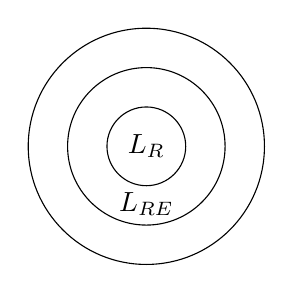
\begin{tikzpicture}
\draw (0,0) circle (0.5cm);
\draw (0,0) circle (1cm);
\draw (0,0) circle (1.5cm);
\node at (0,0) {$L_{\tx{R}}$};
\node at (0,-1cm) [above] {$L_{\tx{RE}}$};
\end{tikzpicture}
\end{center}
\Mark{Definition 5.7}
\end{fdefinition}

\section{Berechenbarkeit}
\Mark{Section 5.5}
\subsection{Die Methode der Diagonalisierung}
\Mark{Subsection 5.5.1}
\begin{ziel}
Nachweis der Existenz von Sprachen, die nicht rekursiv aufz�hlbar sind.
\end{ziel}
Um dies zu zeigen werden wir folgende quantitative �quivalente Aussage beweisen.
\begin{quote}
\ggq{Die M�chtigkeit der Menge aller \ac{TM} ist kleiner als die M�chtigkeit aller Sprachen �ber $\SigB$.}
\end{quote}
Kodierung von Turingmaschinen (Ziel: Nummerierung \ac{bzw.} Ordnung von Turingmaschinen).\\
Sei $M = \rkl{Q, \Sigma, \Gamma, \delta, q_0, \qacc, \qrej}$ eine \ac{TM} mit
\begin{itemize}
\item $Q = \gklamm{q_1, \dots, q_m, q_0, \qacc, \qrej}$
\item $\Gamma = \gklamm{a_1, \dots, a_r}$
\end{itemize}
Die Kodierung der einzelnen Symbole legen wir wie folgt fest
\begin{multicols}{2}
\begin{itemize}
\item $\Code{(q_i)} = 1 0^i 1$ f�r $i = 1 \dots m$
\item $\Code{(q_0)} = 1 0^{m + 1} 1$
\item $\Code{(\qacc)} = 1 0^{m + 2} 1$
\item $\Code{(\qrej)} = 1 0^{m + 3} 1$
\item $\Code{(a_j)} = 11 0^j 11$ $j = 1 \dots r$
\item $\Code{(N)} = 111 0 111$
\item $\Code{(R)} = 111 00 111$
\item $\Code{(L)} = 111 000 111$
\end{itemize}
\end{multicols}
Transitionen werden wie folgt kodiert
\begin{itemize}
\item $\Code{\rkl{\delta (p, a) = (q, b, \alpha)}} =$
		\[\sharp \Code{(p)} \Code{(a)} \Code{(q)} \Code{(b)} \Code{(\alpha)} \sharp\]
\end{itemize}
Eine vollst�ndige \ac{TM} kann dann so kodiert werden:
\[\Code{(M)} = \sharp 0^{m + 3} \sharp 0^r \sharp \Code{(\tx{Transition 1})} \sharp \Code{(\tx{Transition 2})} \dots\]
\begin{fdefinition}
F�r jede \ac{TM} $M$ bezeichnet
\[\Kod{(M)} = \mathcal{h} \rkl{\Code{(M)}}\]
die Kodierung von $M$, wobei $\mathcal{h}$ Homomorphismus mit $\mathcal{h} (0) = 00$, $\mathcal{h} (1) = 11$ und $\mathcal{\sharp} = 10$.
\[\Kod{(TM)} = \gklamm{\Kod{(M)} \vert M \tx{ ist \ac{TM}}}\]
bezeichnet die Menge der Kodierungen aller \ac{TM}.
\end{fdefinition}
